\documentclass[12pt]{article}
\usepackage[margin=1in]{geometry}                % See geometry.pdf to learn the layout options. There are lots.
\geometry{letterpaper}                   % ... or a4paper or a5paper or ... 
%\geometry{landscape}                % Activate for for rotated page geometry
\usepackage[parfill]{parskip}    % Activate to begin paragraphs with an empty line rather than an indent

%%%%%%%%%%%%%%%%%%%%
\newcommand{\hide}[1]{}
\setcounter{tocdepth}{4}
\usepackage{natbib}
\usepackage{xcolor}
\usepackage{url}
\usepackage{hyperref}
\usepackage{mathtools}
\usepackage[utf8]{inputenc}


\hide{
\usepackage{amscd}
\usepackage{amsfonts}
\usepackage{amsmath}
\usepackage{amssymb}
\usepackage{amsthm}
\usepackage{cases}		 
\usepackage{cutwin}
\usepackage{enumerate}
\usepackage{enumitem}
\usepackage{epstopdf}
\usepackage{graphicx}
\usepackage{ifthen}
\usepackage{lipsum}
\usepackage{mathrsfs}	
\usepackage{multimedia}
\usepackage{wrapfig}
}
\bibliographystyle{humanbio}

\usepackage{caption}
\usepackage[utf8]{inputenc}

\usepackage{listings}
\usepackage{xcolor}
\lstset{language=[LaTeX]TeX,breaklines=true} % Word wrap within listings environment
\definecolor{codegreen}{rgb}{0,0.6,0}
\definecolor{codegray}{rgb}{0.5,0.5,0.5}
\definecolor{codepurple}{rgb}{0.58,0,0.82}
\definecolor{backcolour}{rgb}{0.95,0.95,0.92}

\lstdefinestyle{mystyle}{
    backgroundcolor=\color{backcolour},   
    commentstyle=\color{codegreen},
    keywordstyle=\color{magenta},
    numberstyle=\tiny\color{codegray},
    stringstyle=\color{codepurple},
    basicstyle=\ttfamily\footnotesize,
    breakatwhitespace=false,         
    breaklines=true,                 
    captionpos=b,                    
    keepspaces=true,                 
    numbers=left,                    
    numbersep=5pt,                  
    showspaces=false,                
    showstringspaces=false,
    showtabs=false,                  
    tabsize=2
}
\lstset{style=mystyle,columns=fullflexible}

\newcommand{\itemlist}[1]{\begin{itemize}#1\end{itemize}}
\newcommand{\enumlist}[1]{\begin{enumerate}#1\end{enumerate}}
\newcommand{\desclist}[1]{\begin{description}#1\end{description}}
\newcommand\tab[1][0.5cm]{\hspace*{#1}}

\newcommand{\Answer}[1]{\begin{quote}{\color{blue}#1}\end{quote}}
\newcommand{\AND}{\wedge}
\newcommand{\OR}{\vee}
\newcommand{\ra}{\rightarrow}
\newcommand{\lra}{\leftrightarrow}

\title {{\bf Using Git with Vivado} \\
\large{University of Arizona Fall 2020 ECE 274A Digital Logic}}

\author{Mitchell Dzurick}
\date{8/24/2020}
\begin{document}

\maketitle

\tableofcontents
\listoffigures
\clearpage


\section{Overview} \label{Overview}
This guide will provide supplementary information for ECE 274A Lab section. This guide will be extremely useful for managing and storing the source code of your project. This guide will assume no prior knowledge of git or bash is known. The two major concepts that this guide will explain are the following:
\begin{enumerate}
    \item basic git usage
    \item basic bash usage
\end{enumerate}

This guide will most likely use language that you may not be familiar with. Most things are explained thoroughly but if you are not exactly sure what a word means you are encouraged to look it up or ask on Piazza!

\textbf{NOTE: This is not information you will be tested on, but rather information that will be helpful in this class and your future career as an engineer.}

\section{Intro to Git and Bash} \label{Intro to Git}
\subsection{What is Git?}
Git is a very common \textbf{VCS (Version Control Software)} that you will see in industry. Git has an emphasis on speed, data integrity and distributed workloads. All VCS systems generally have a similar goal of tracking changes in files and storing data on a remote server.

You can learn all about git through their official website \href{https://git-scm.com/}{https://git-scm.com/}. The book "Pro Git" is also completely free to view through your browser \href{https://git-scm.com/book/en/v2}{https://git-scm.com/book/en/v2}.

\subsection{What is Bash?}
Bash is an acronym that stands for Bourne Again SHell. Bash is the unix shell that GNU Project maintains. A unix shell is simply just a command-line interpreter that sends commands directly to the operating system. You can think of Bash simply as your terminal.

\begin{center}
    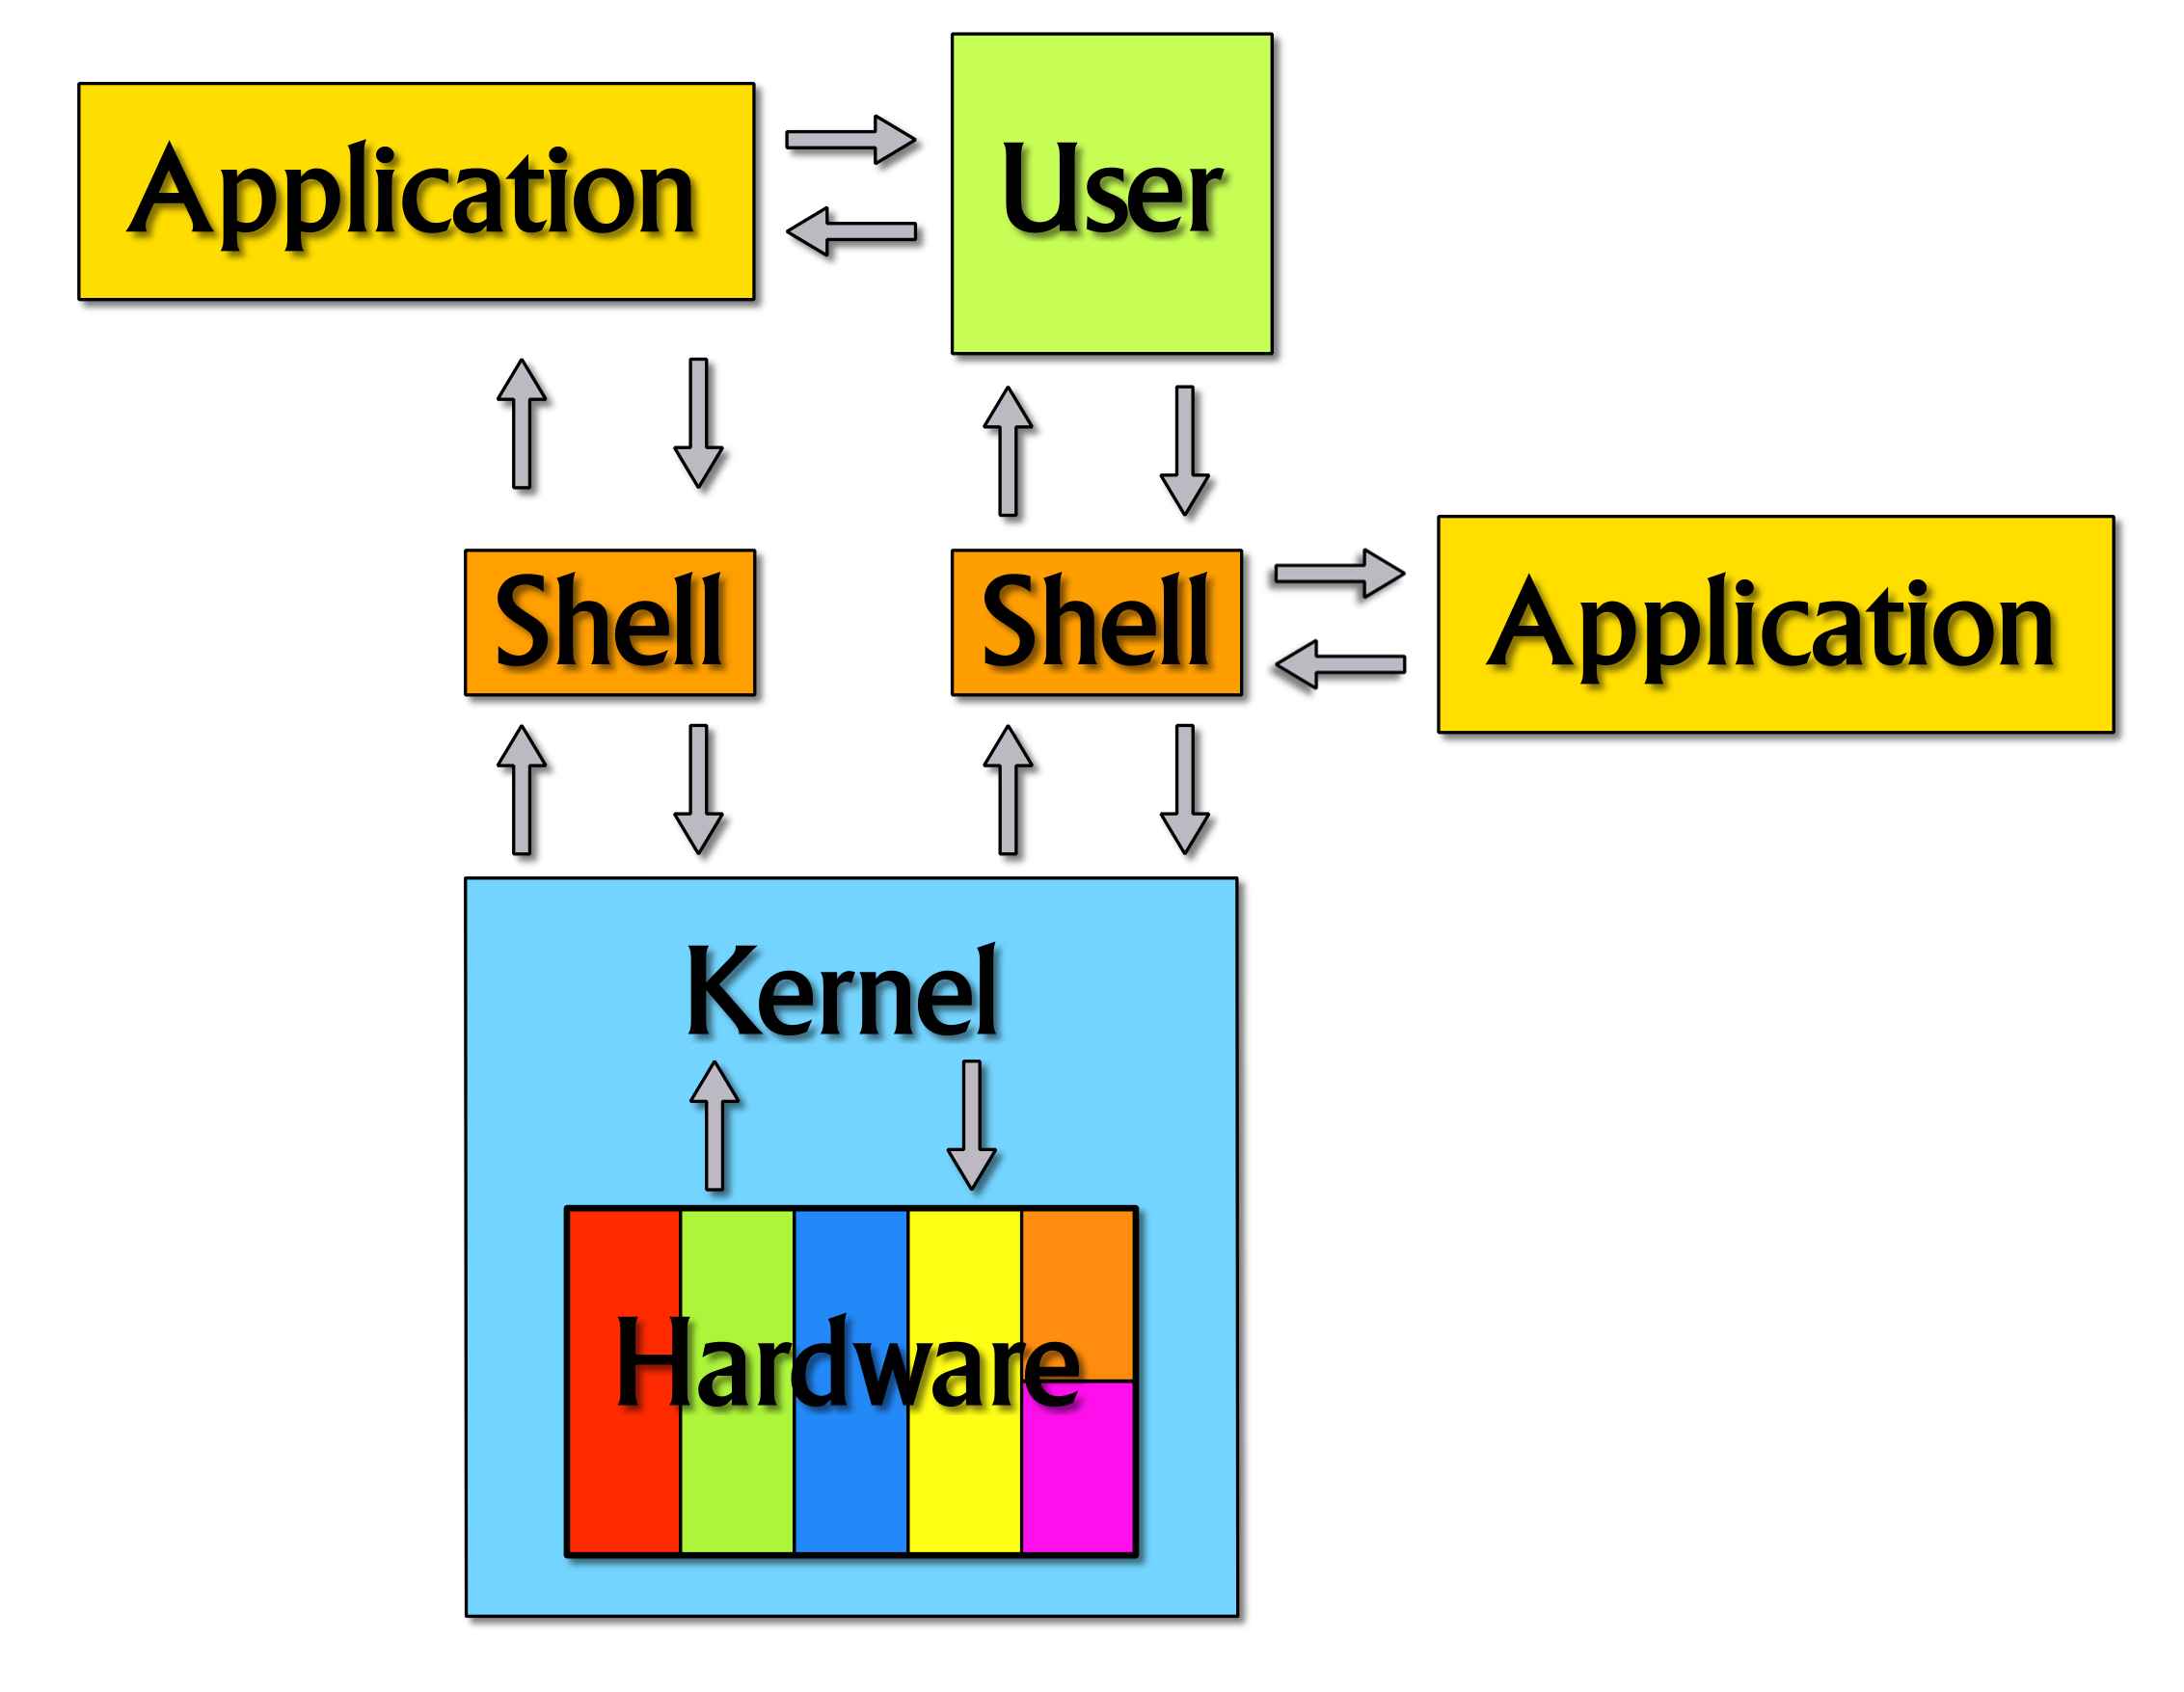
\includegraphics[scale=0.4]{Flow1.jpg}
    \captionof{figure}{Command Flow}
    \label{fig:user_flow}
\end{center}

Figure~\ref{fig:user_flow} is a diagram provided from opensuse at \href{https://en.opensuse.org/images/e/e2/Flow1.jpg}{https://en.opensuse.org/images/e/e2/Flow1.jpg} which goes deeper into how the user interacts with the system. You as the User will send commands to the Kernel using a Shell (in our case, Bash), where the Kernel then controls the Hardware. Think of the Kernel as a resource manager for hardware.

\section{Using Git with Windows} \label{Using Git with Windows}
Windows does not have a git client by default, so we will need to download software for that. This guide will utilize the popular \emph{git for windows}, or better known as Git Bash.
\subsection{Git Bash}
\subsubsection{Installation} \label{Win10-GitBashInstall}
On the Lab PC, enter the website \url{https://gitforwindows.org/} and click "Download". Once the download is finished, open the installer. All of the default options are good, sane options, so just keep clicking "Next" Until the installation is done.
\subsubsection{Using Git Bash}
When you are finished downloading Git Bash from Section \ref{Win10-GitBashInstall}, you can open up Git Bash by typing in "git bash" after pressing the windows key. Upon pressing enter, you will be greeted with a terminal that looks like the Figure~\ref{fig:win_06_Git_Bash}.

\begin{center}
    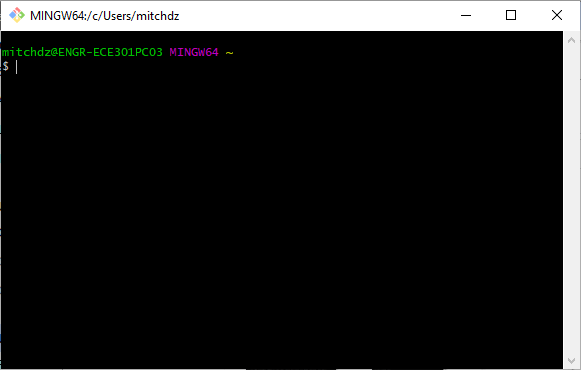
\includegraphics[scale=0.6]{win_06_Git_Bash.PNG}
    \captionof{figure}{Git Bash Default Screen}
    \label{fig:win_06_Git_Bash}
\end{center}

Now that you are in the terminal, you can use any commands that any usual bash terminal would have. You can enter the following command \textbf{(do not type the \$ at the start of the command, that is there by default)}:

\begin{lstlisting}
$ echo $PWD
\end{lstlisting}

\begin{center}
    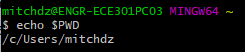
\includegraphics[width=3in]{win_07_echo_PWD.PNG}
    \captionof{figure}{Printing CWD in Git Bash}
    \label{fig:win_07_echo_PWD}
\end{center}

Figure~\ref{fig:win_07_echo_PWD} shows the result of running the above command. The result is "/c/Users/mitch". /c/ refers to the hard drive. "Users/mitch" refers to the path on that hard drive. The reason that you see the yellow tilde (that is the $\sim$ character), is that \textbf{$\sim$ is shorthand for "/c/Users/mitch"} (your username will show up instead of mitch).

You can change your directory into a folder where we can clone our repository. For this, we will be using the \textbf{cd} command. You can think of \textbf{cd} as standing for "Change Directory". Execute the following:

\begin{lstlisting}
$ cd Documents/
\end{lstlisting}

\begin{center}
    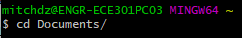
\includegraphics[width=3in]{win_08_cd_Doc.PNG}
    \captionof{figure}{Changing Directory to Documents}
    \label{fig:win_08_cd_Doc}
\end{center}

Figure~\ref{fig:win_08_cd_Doc} shows the results of changing our directory to Documents. You can now note that the yellow text says "$\sim$/Documents" which is actually referring to "/c/Users/mitch/Documents" in my case because the name for my User is mitch.

Let's create our own directory called 'git' in $\sim$Documents. This is where we will clone our git repository to be used for later.

\begin{lstlisting}
$ mkdir git
$ cd git
\end{lstlisting}

now you will be located in $\sim$/Documents/git. From here, let's clone a reference repository just to test everything. Execute the following command to clone an example repository with some Verilog code.

\begin{lstlisting}
$ git clone https://github.com/mitchdz/ExampleVerilogCode
\end{lstlisting}

Now you have cloned a repository into your Documents folder that you will be able to see. In the terminal we can enter the new cloned repository and view the files with the \textbf{ls} command.

\begin{lstlisting}
$ cd ExampleVerilogCode
$ ls -l
$ ls src/
\end{lstlisting}

\begin{center}
    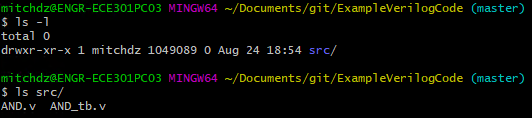
\includegraphics[width=6in]{win_bash_clone_2.PNG}
    \captionof{figure}{viewing the example Github repo}
    \label{fig:win_bash_clone_2}
\end{center}

Figure~\ref{fig:win_bash_clone_2} shows the results of the directory. We notice that one file exists named "src/". The blue name and the trailing "/" indicates that src is a directory. We can list the contents of the directory as shown in the same figure with "ls src/", where we see two files; AND.v and AND{\_}tb.v

Now let's create a Vivado project that imports this folder. Open up Vivado and click Create a Project as shown in Figure~\ref{fig:Vivado 2019.2.1 Default Screen}

\begin{center}
    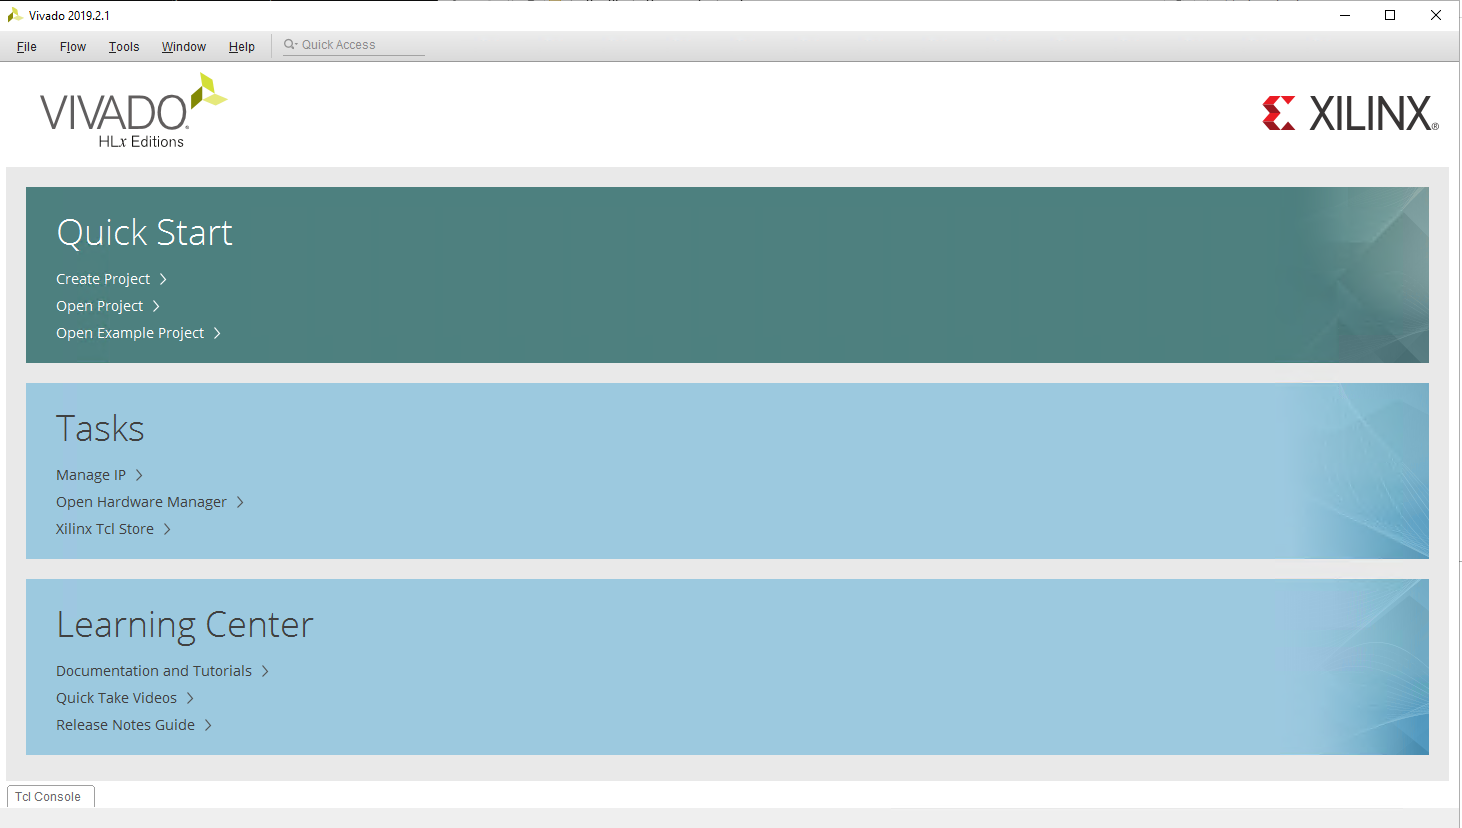
\includegraphics[scale=0.3]{viv_01.PNG}
    \captionof{figure}{Vivado 2019.2.1 Default Screen}
    \label{fig:Vivado 2019.2.1 Default Screen}
\end{center}

Name the Project "testGitExample" as shown in Figure~\ref{fig:Naming Example Project}

\begin{center}
    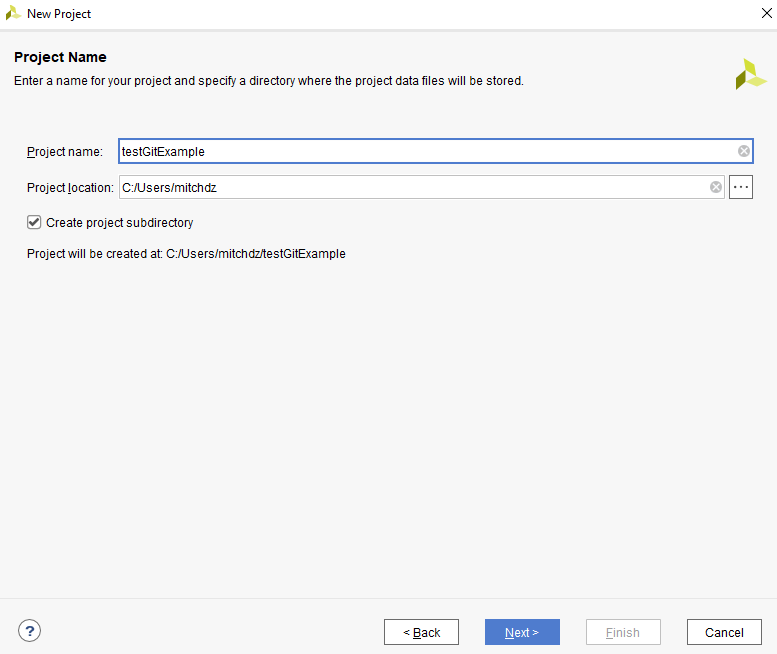
\includegraphics[scale=0.4]{viv_02.PNG}
    \captionof{figure}{Naming Example Project}
    \label{fig:Naming Example Project}
\end{center}

\begin{center}
    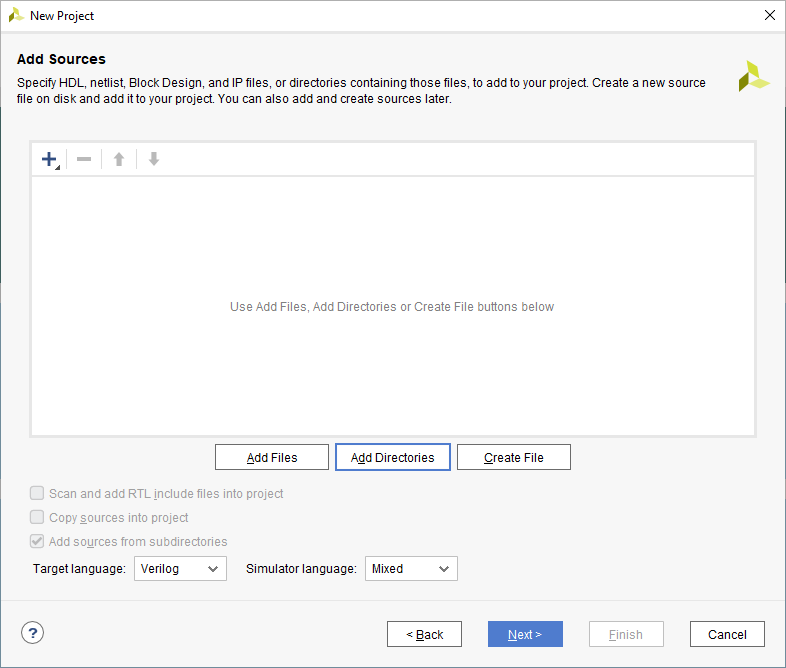
\includegraphics[scale=0.6]{viv_03.PNG}
    \captionof{figure}{Adding Sources Page}
    \label{fig:Adding Sources Page}
\end{center}

Choose RTL Project and then when it asks you to choose your sources, choose to 'Add Directories'. Figure~\ref{fig:Adding Sources Page} shows the window to select sources.

\begin{center}
    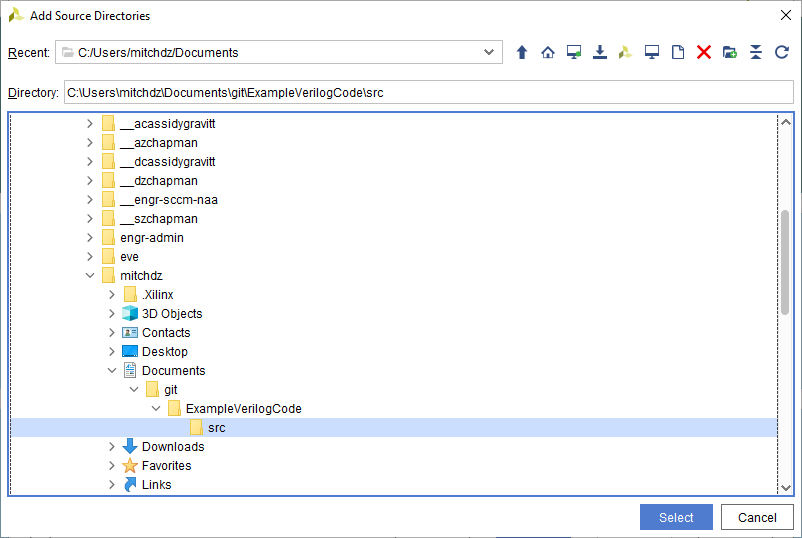
\includegraphics[scale=0.6]{viv_04.PNG}
    \captionof{figure}{Adding Example Code into Vivado}
    \label{fig:Adding Example Code into Vivado}
\end{center}

\textbf{select the src/ directory of the ExampleVerilogCode just like how Figure~\ref{fig:Adding Example Code into Vivado} shows.} Once you press Select, Vivado will pull this code into the project, and any changes made to this code will also be changed here. This allows us to easily source control the code because all of the modified code will be in a git directory.

Keep Pressing 'Next' And then you will get into the Vivado Project Manager as shown in Figure~\ref{fig:Vivado Project Manager}

\begin{center}
    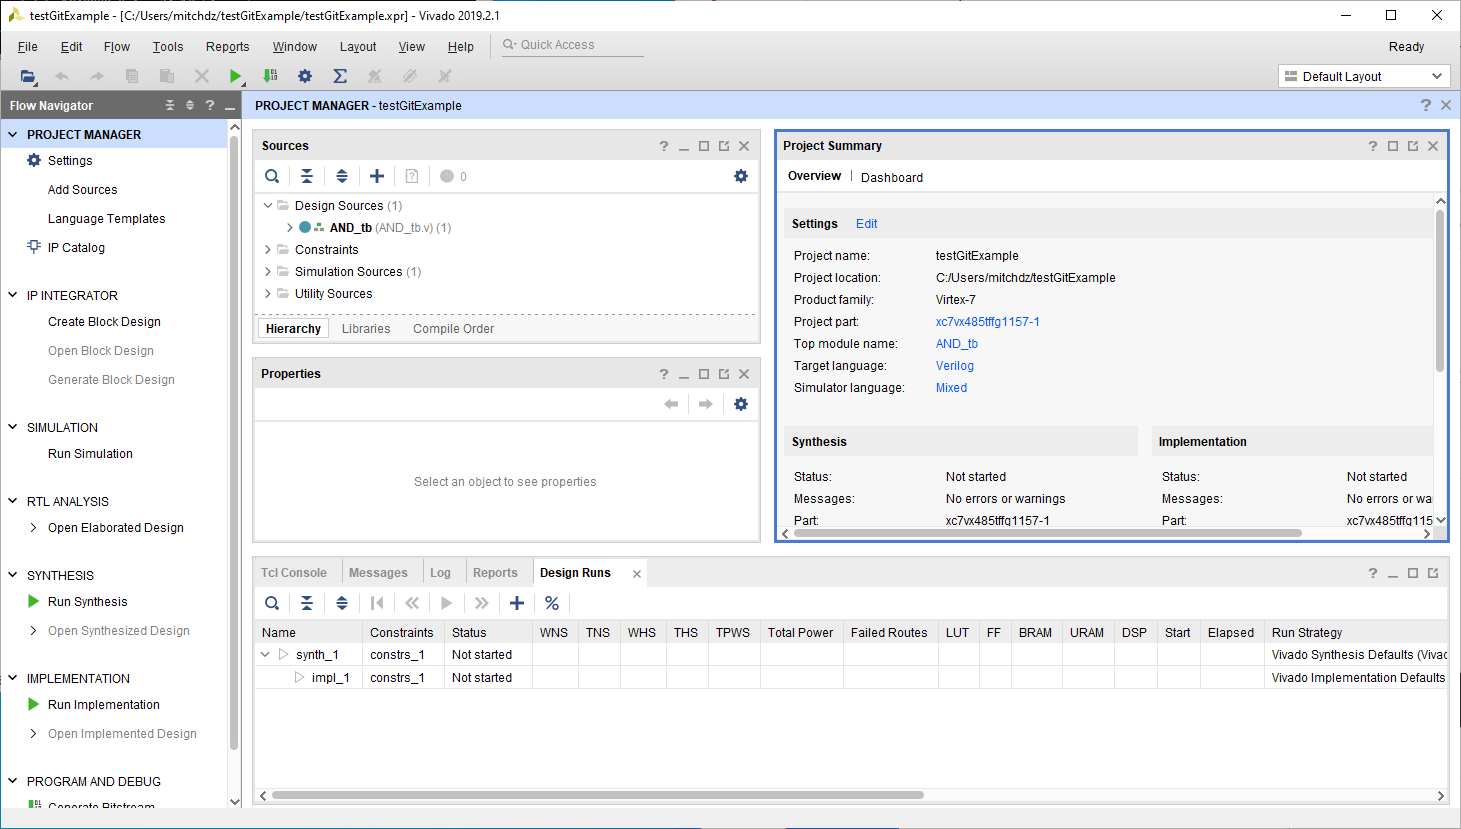
\includegraphics[scale=0.4]{viv_05.PNG}
    \captionof{figure}{Vivado Project Manager}
    \label{fig:Vivado Project Manager}
\end{center}

Once you get into the Vivado Project Manager wait until you can see AND{\_}tb in the Design Sources section as shwon in Figure~\ref{fig:Vivado Project Manager}. After that file shows up, press 'Run Simulation' on the left side. This will take a little bit.

\begin{center}
    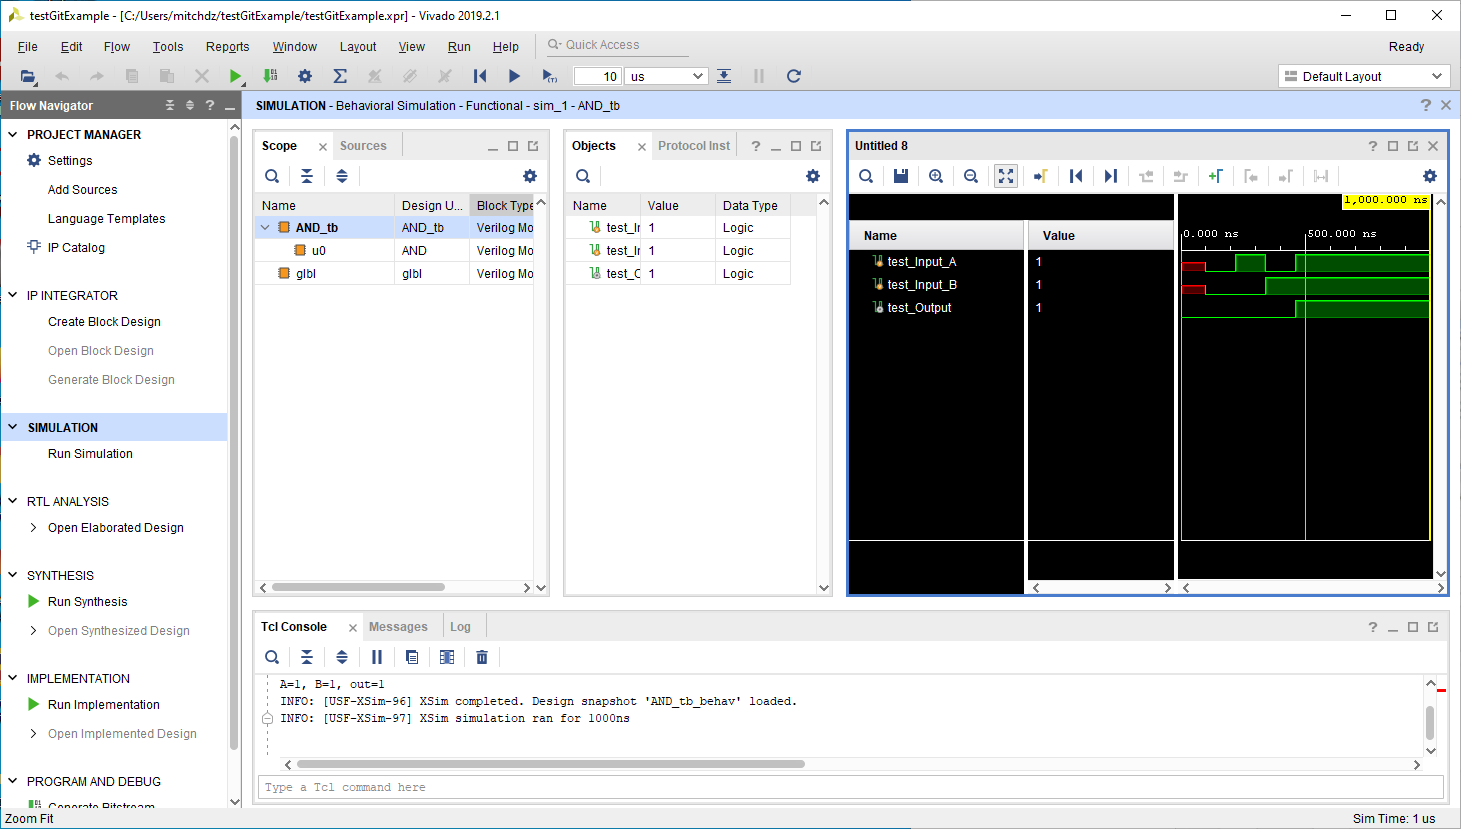
\includegraphics[scale=0.4]{viv_06.PNG}
    \captionof{figure}{Running Simulation of Example Project}
    \label{fig:Running Simulation of Example Project}
\end{center}

After the Simulation is done, you will see Figure~\ref{fig:Running Simulation of Example Project}. Click the "Zoom fit" button as shown being highlighted in the figure to be able to see the waveform better. The component being tested is an AND gate, so the results should make sense!

Let's make a change in the source code and see how to upload that to github.

\begin{center}
    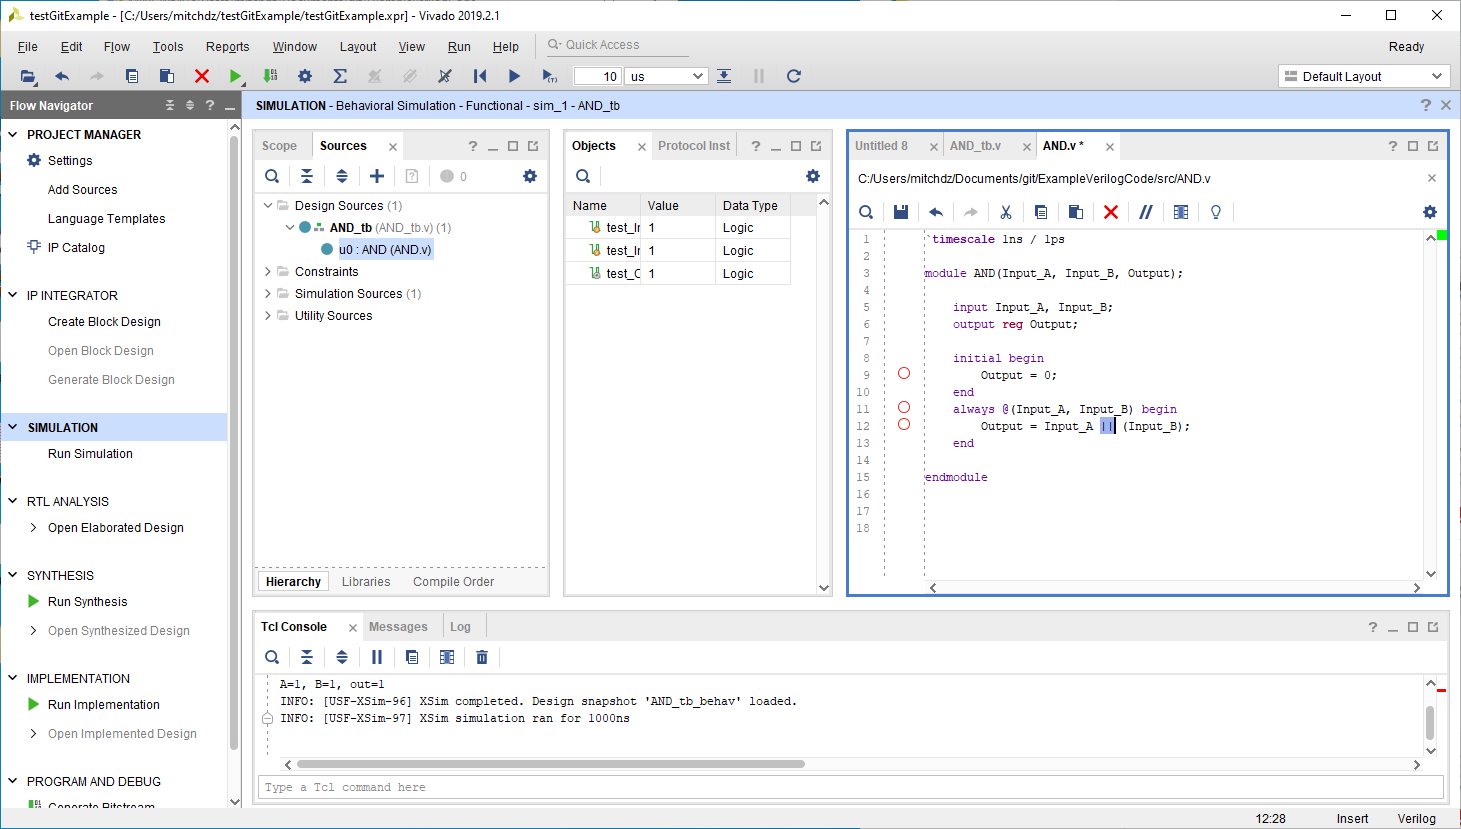
\includegraphics[scale=0.4]{viv_07.PNG}
    \captionof{figure}{Modifying Example Source Code}
    \label{fig:Modifying Example Source Code}
\end{center}

Click the "Sources" Tab and then double click u0 as shown in Figure~\ref{fig:Modifying Example Source Code}. Let's change the AND gate to an OR gate. \textbf{Notice that There is a * next to AND.v* in the right highlighted section.}This means there is code that has not been saved. Pressing ctrl + s will save the code and make the asterick go away, then we can see the change in git.

\begin{center}
    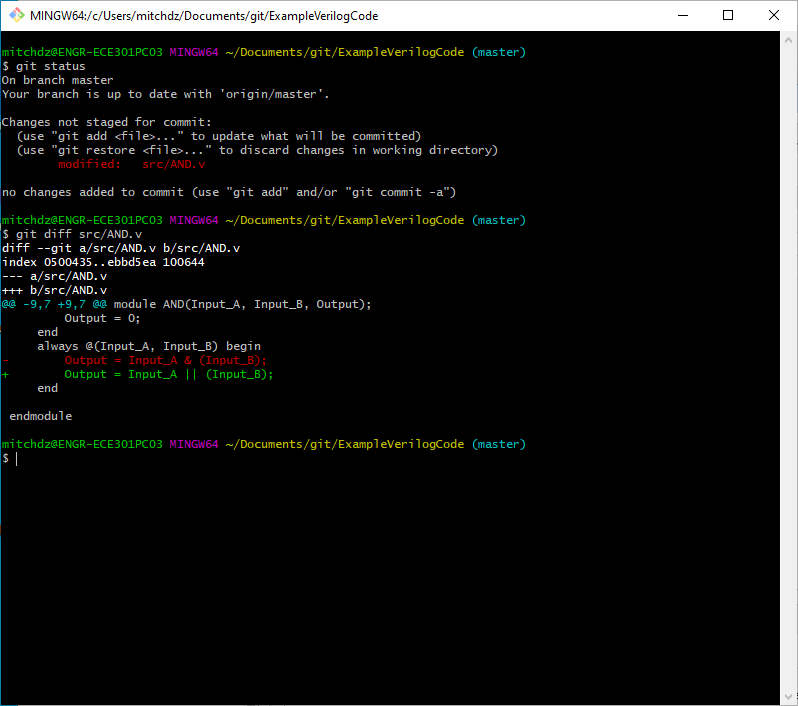
\includegraphics[scale=0.8]{viv_08.PNG}
    \captionof{figure}{Viewing Modified Source Code in Git}
    \label{fig:Viewing Modified Source Code in Git}
\end{center}

Go back to Git Bash to check out the file changes. If you closed Git Bash and need to get back to the directory simply type "cd ~/Documents/git/ExampleVerilogCode". If not you can view the changes using git status and git diff as shown in Figure~\ref{fig:Viewing Modified Source Code in Git}.

\begin{lstlisting}
$ git status
$ git diff src/AND.v
\end{lstlisting}

So now we have a file that can be uploaded to git. The workflow for this as commands is as follows:

\begin{lstlisting}
$ git add src/AND.v
$ git commit -m 'this text is the commit message text'
$ git push
\end{lstlisting}

You won't be able to execute the last command because this repository does not belong to you. Proceed to Section \ref{Creating your own Github Repository} in order to create your own repo and test this out!

To recap, all you need to do in order to make the code appear from the computer to Github is:

\begin{lstlisting}
$ git status # to check which files have changed
$ git add <file(s) to be commited>
$ git commit -m 'this text is the commit message text'
$ git push
\end{lstlisting}






\clearpage
\section{Creating your own Github Repository} \label{Creating your own Github Repository}
There is a lot of software that utilizes git such as GitHub, SourceForge, Bitbucket and GitLab. For this guide we will utilize Github. To get some cool bonuses for being a student you can even register for the student pack at \href{https://education.github.com/pack}{https://education.github.com/pack}.

\begin{center}
    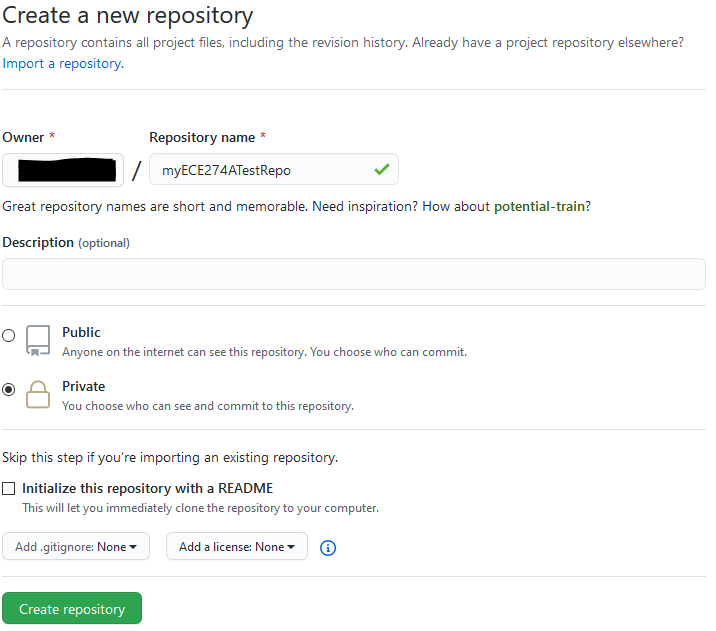
\includegraphics[scale=0.8]{git_test_0.PNG}
    \captionof{figure}{Creating a new Github Repo}
    \label{fig:Creating a new Github Repo}
\end{center}

Go to your Github account after you create it and then click "New Project". You will be greeted with Figure~\ref{fig:Creating a new Github Repo}. Name your repository whatever you want, but make sure that "Private" is selected. By default, repositories are Public. If you accidentally create a Public Repo it can be changed in Settings > Options > Change repository visibility.

After creating the repo, follow the steps from Section \ref{Using Git with Windows} with your own repository. Just copy the ExampleVerilogCode over to your new repository. An example of this is shown below in Figure~\ref{fig:adding Example Code to Personal Repo and Pushing}

\begin{center}
    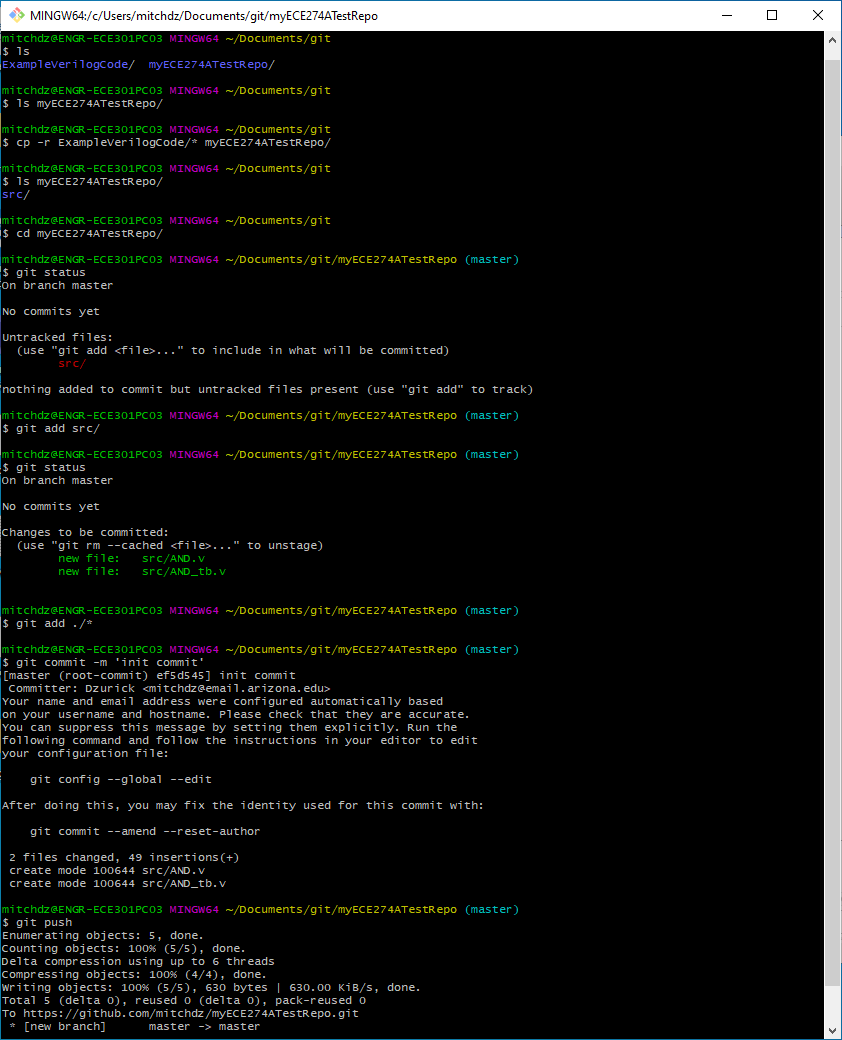
\includegraphics[scale=0.8]{viv_10.PNG}
    \captionof{figure}{adding Example Code to Personal Repo and Pushing}
    \label{fig:adding Example Code to Personal Repo and Pushing}
\end{center}


To review Figure~\ref{fig:adding Example Code to Personal Repo and Pushing}, the following commands are used:

\begin{lstlisting}
$ cp -r ExampleVerilogCode/* myECE274ATestRepo/
$ cd myECE274ATestRepo
$ git status
$ git add ./*
$ git commit -m 'init commit'
$ git push
\end{lstlisting}

Line 1 uses the cp command, which you can think of as "copy". This command copies the contents of ExampleVerilogCode into myECE274ATestRepo. Line 4 uses something new which is the *. The * is a special character called a wildcard. The * refers to matching any string, so what Line 4 is doing is adding every file in the directory to git.

\section{Adding files in Vivado}
Say you need to add a file in Vivado, but want that file to appear in your git directory. No problem!

In Vivado go to File > Add Sources.. (or the shortcut Alt + A). Click \textbf{Add or create design sources}. 

\begin{center}
    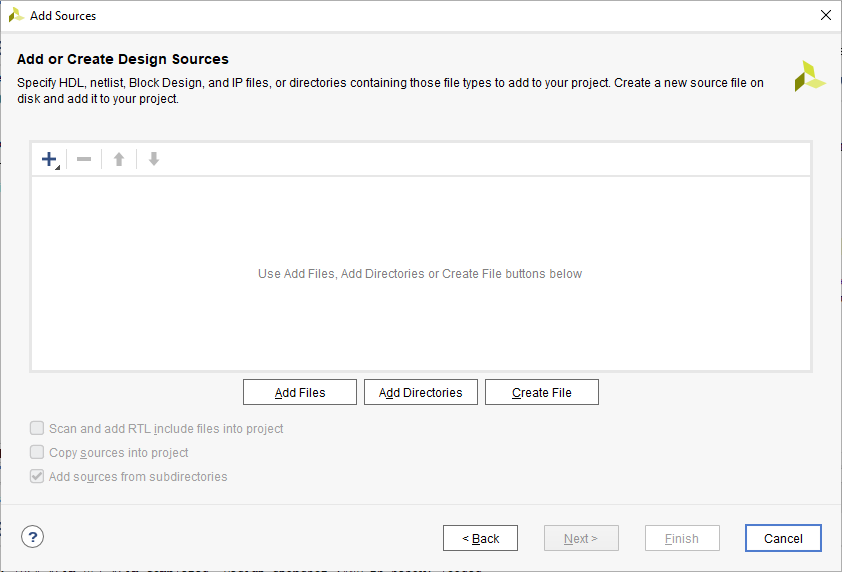
\includegraphics[scale=0.5]{viv_11.PNG}
    \captionof{figure}{Adding Sources in Verilog}
    \label{fig:Adding Sources in Verilog part 2}
\end{center}

Click "Create File" in Figure~\ref{fig:Adding Sources in Verilog part 2}.

\begin{center}
    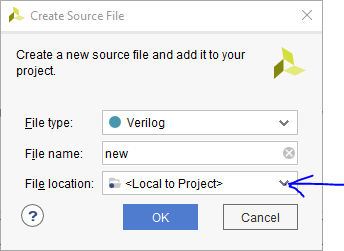
\includegraphics[scale=0.8]{viv_12.PNG}
    \captionof{figure}{Create Source File Screen}
    \label{fig:Create Source File Screen}
\end{center}

Click the drop down arrow that is being pointed to in Figure~\ref{fig:Create Source File Screen}. Make sure to make a name for this file, in this case the file name is "new".

\begin{center}
    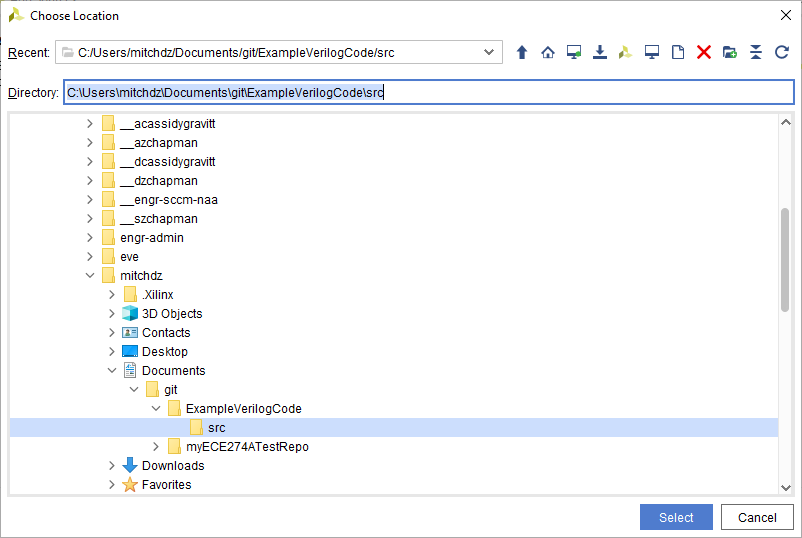
\includegraphics[scale=0.5]{viv_13.PNG}
    \captionof{figure}{Selecting Target Location}
    \label{fig:Selecting Target Location}
\end{center}

Figure~\ref{fig:Selecting Target Location} shows the Location Highlights ~/Documents/git/ExampleVerilogCode/git which was highlighted by default! Simply press Select.

\begin{center}
    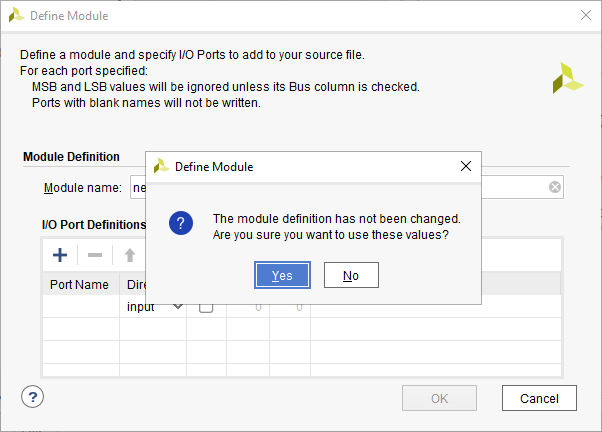
\includegraphics[scale=0.7]{viv_14.PNG}
    \captionof{figure}{Defining Module for New File}
    \label{fig:Defining Module for New File}
\end{center}

You'll need to define a Module for your new file as shown in Figure~\ref{fig:Defining Module for New File}. Just select "OK" and then "Yes". Wait a little bit and your new file will be in your git directory ready to be modified!

One final test...

\begin{center}
    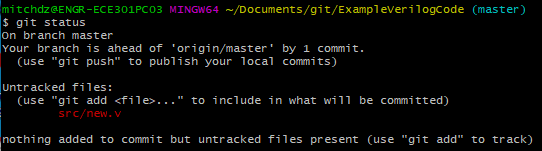
\includegraphics[scale=1.0]{viv_15.PNG}
    \captionof{figure}{Checking For The New File in Git}
    \label{fig:Checking For The New File in Git}
\end{center}

The new file is there!

\end{document}